
\documentclass[a4paper]{jsarticle}
\setlength{\baselineskip}{16pt}
\setlength{\parskip}{6mm}

% Packages
\usepackage[top = 20truemm, bottom = 20truemm, left = 30truemm, right = 30truemm]{geometry}
\usepackage{amsmath} % For mathematical equations
\usepackage{cite} % For citations
\usepackage{hyperref} % For hyperlinks
\usepackage[dvipdfmx]{graphicx}
\usepackage{here} % For figure placement

% Title and author
\title{中級ミクロデータサイエンス期末課題\\Problem Set 3}
\author{横浜国立大学経済学部3年\\学籍番号 2125178\\廣江友哉}

\begin{document}

\maketitle

\section{データセットのシミュレーション}

ソースコードは、\url{https://github.com/tomoyahiroe/replication-project} にある。リポジトリページ下部の README.md ファイルを参照いただきたい。各Problem Set についての説明を記述している。

データセットは以下のように生成した。

\begin{figure}[H]
  \centering
  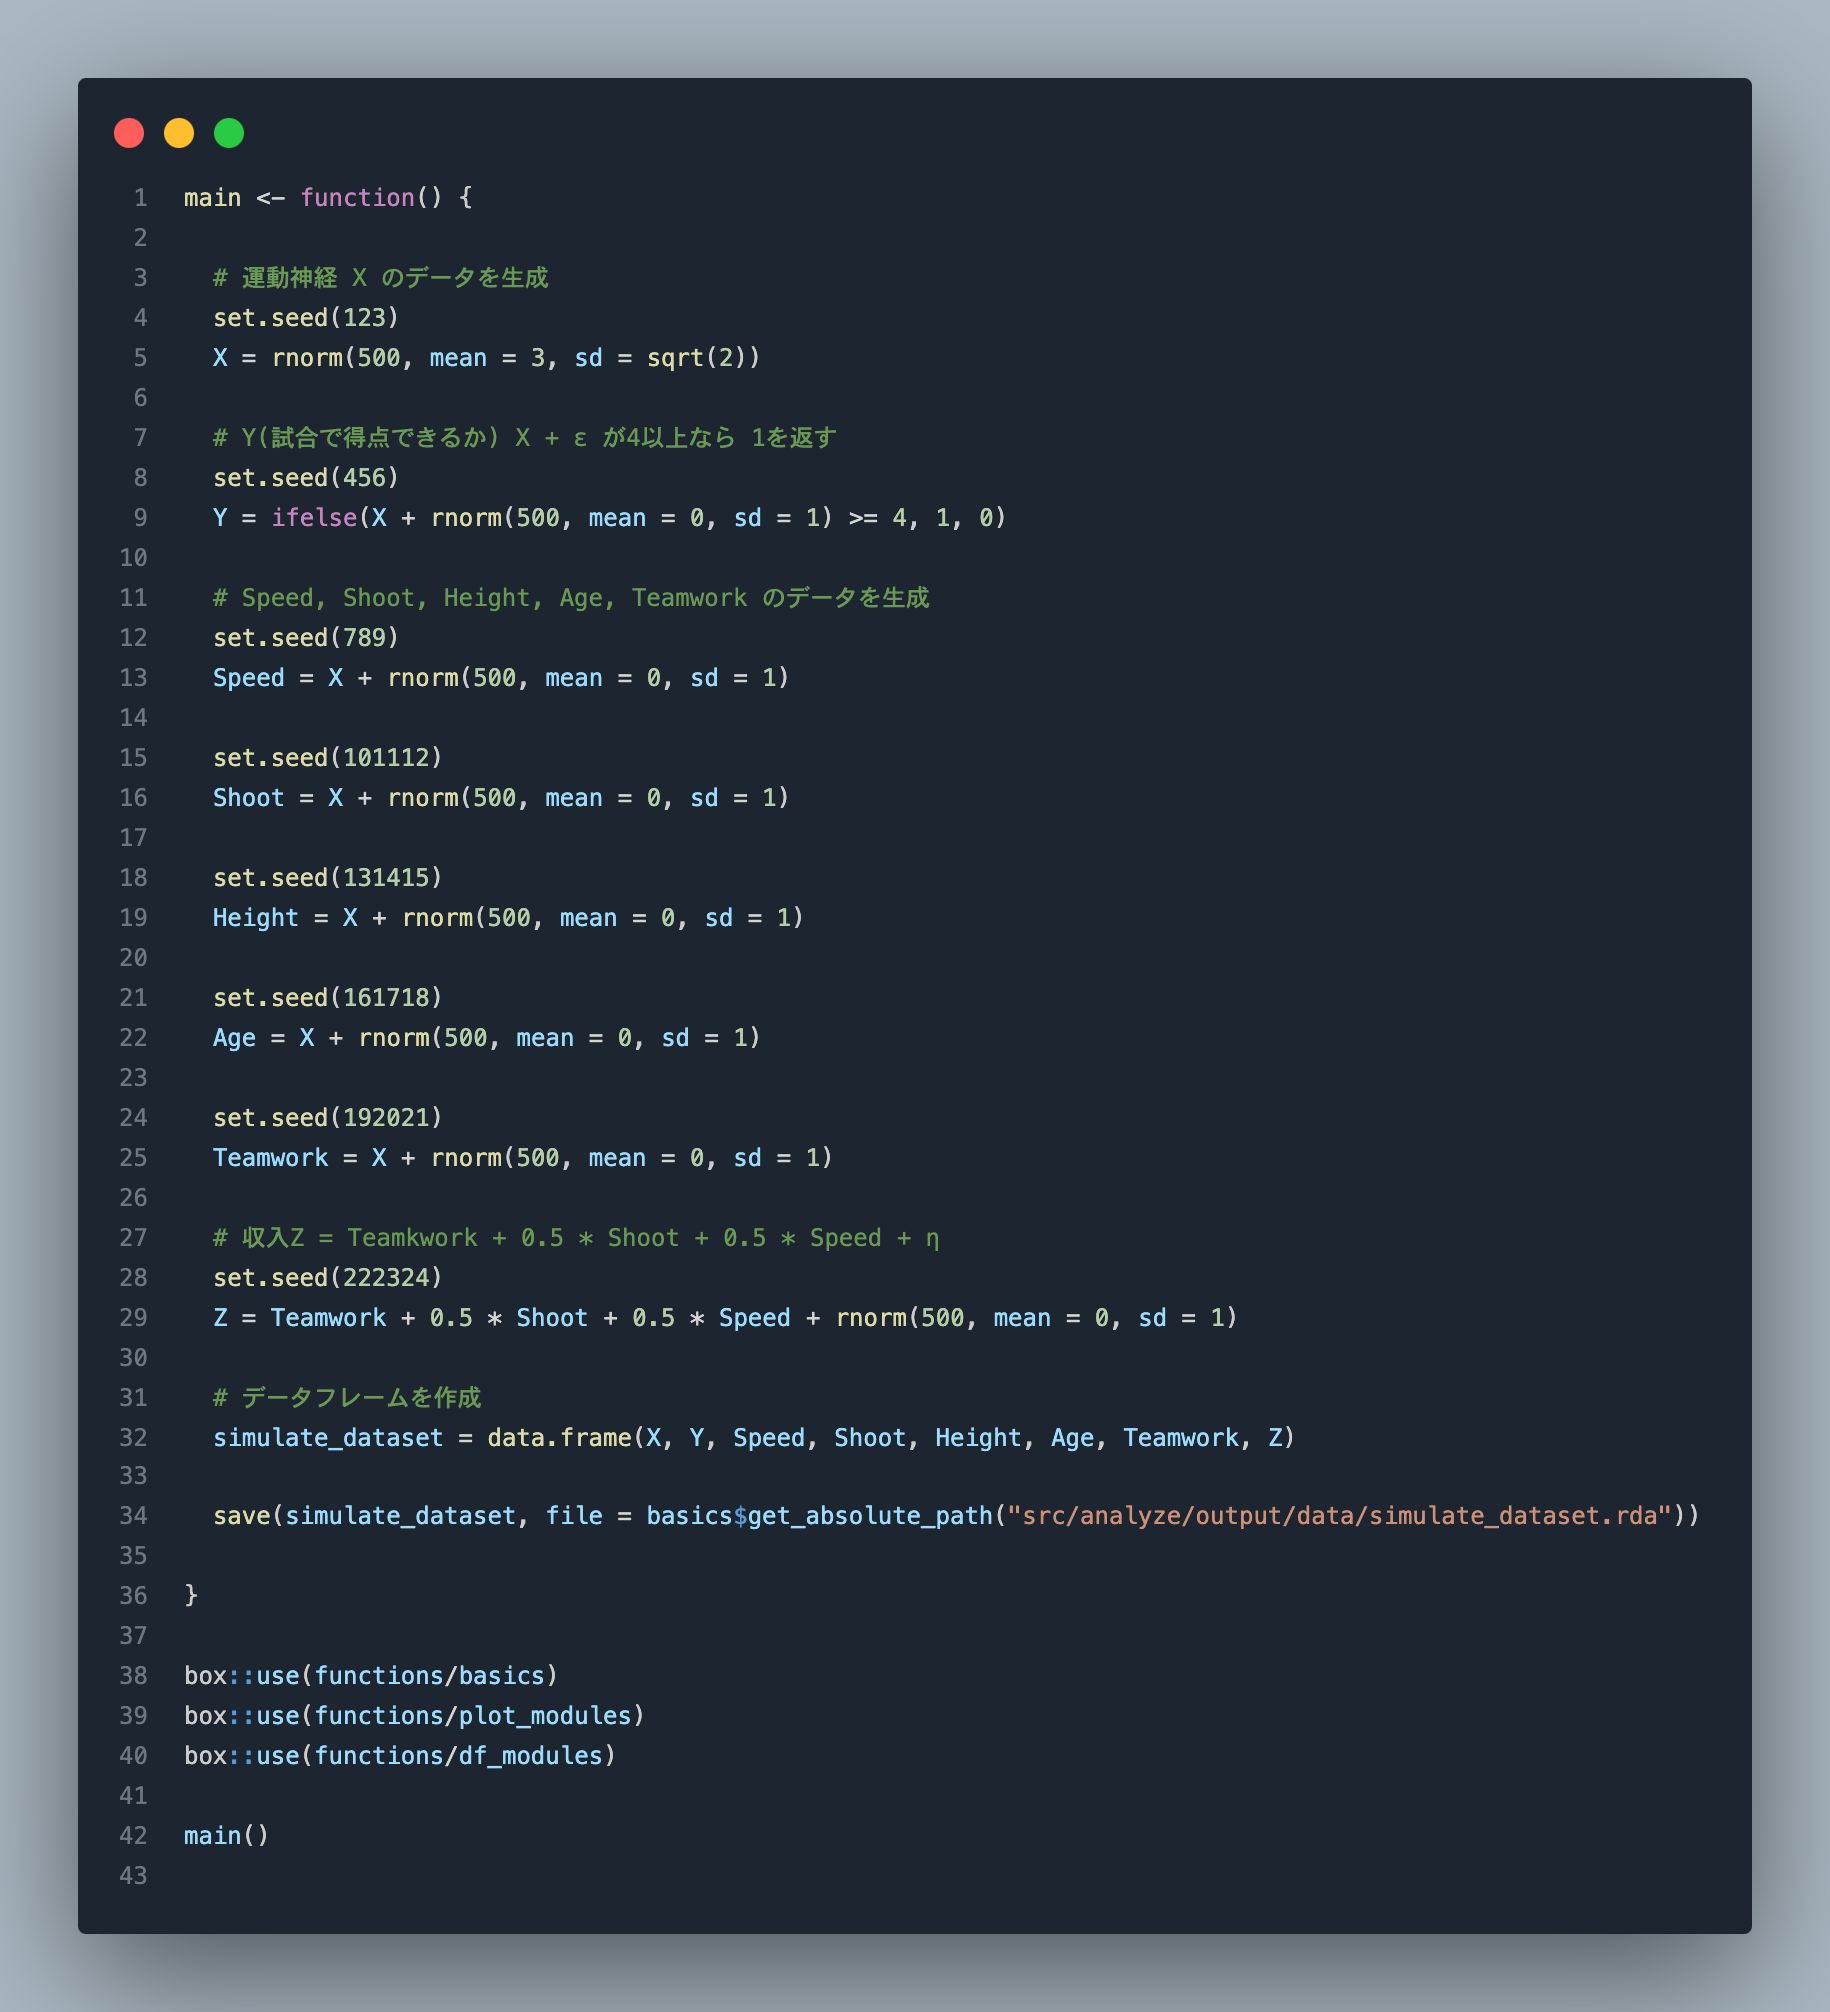
\includegraphics[width = 0.6\hsize]{\$HOME/code_box/learn/R/replication-project/src/analyze/output/simulate_code.png}

\end{figure}


\section{分布の推定}

\subsection{ヒストグラムを用いることの難しさを議論せよ}
\begin{figure}[H]
  \centering
  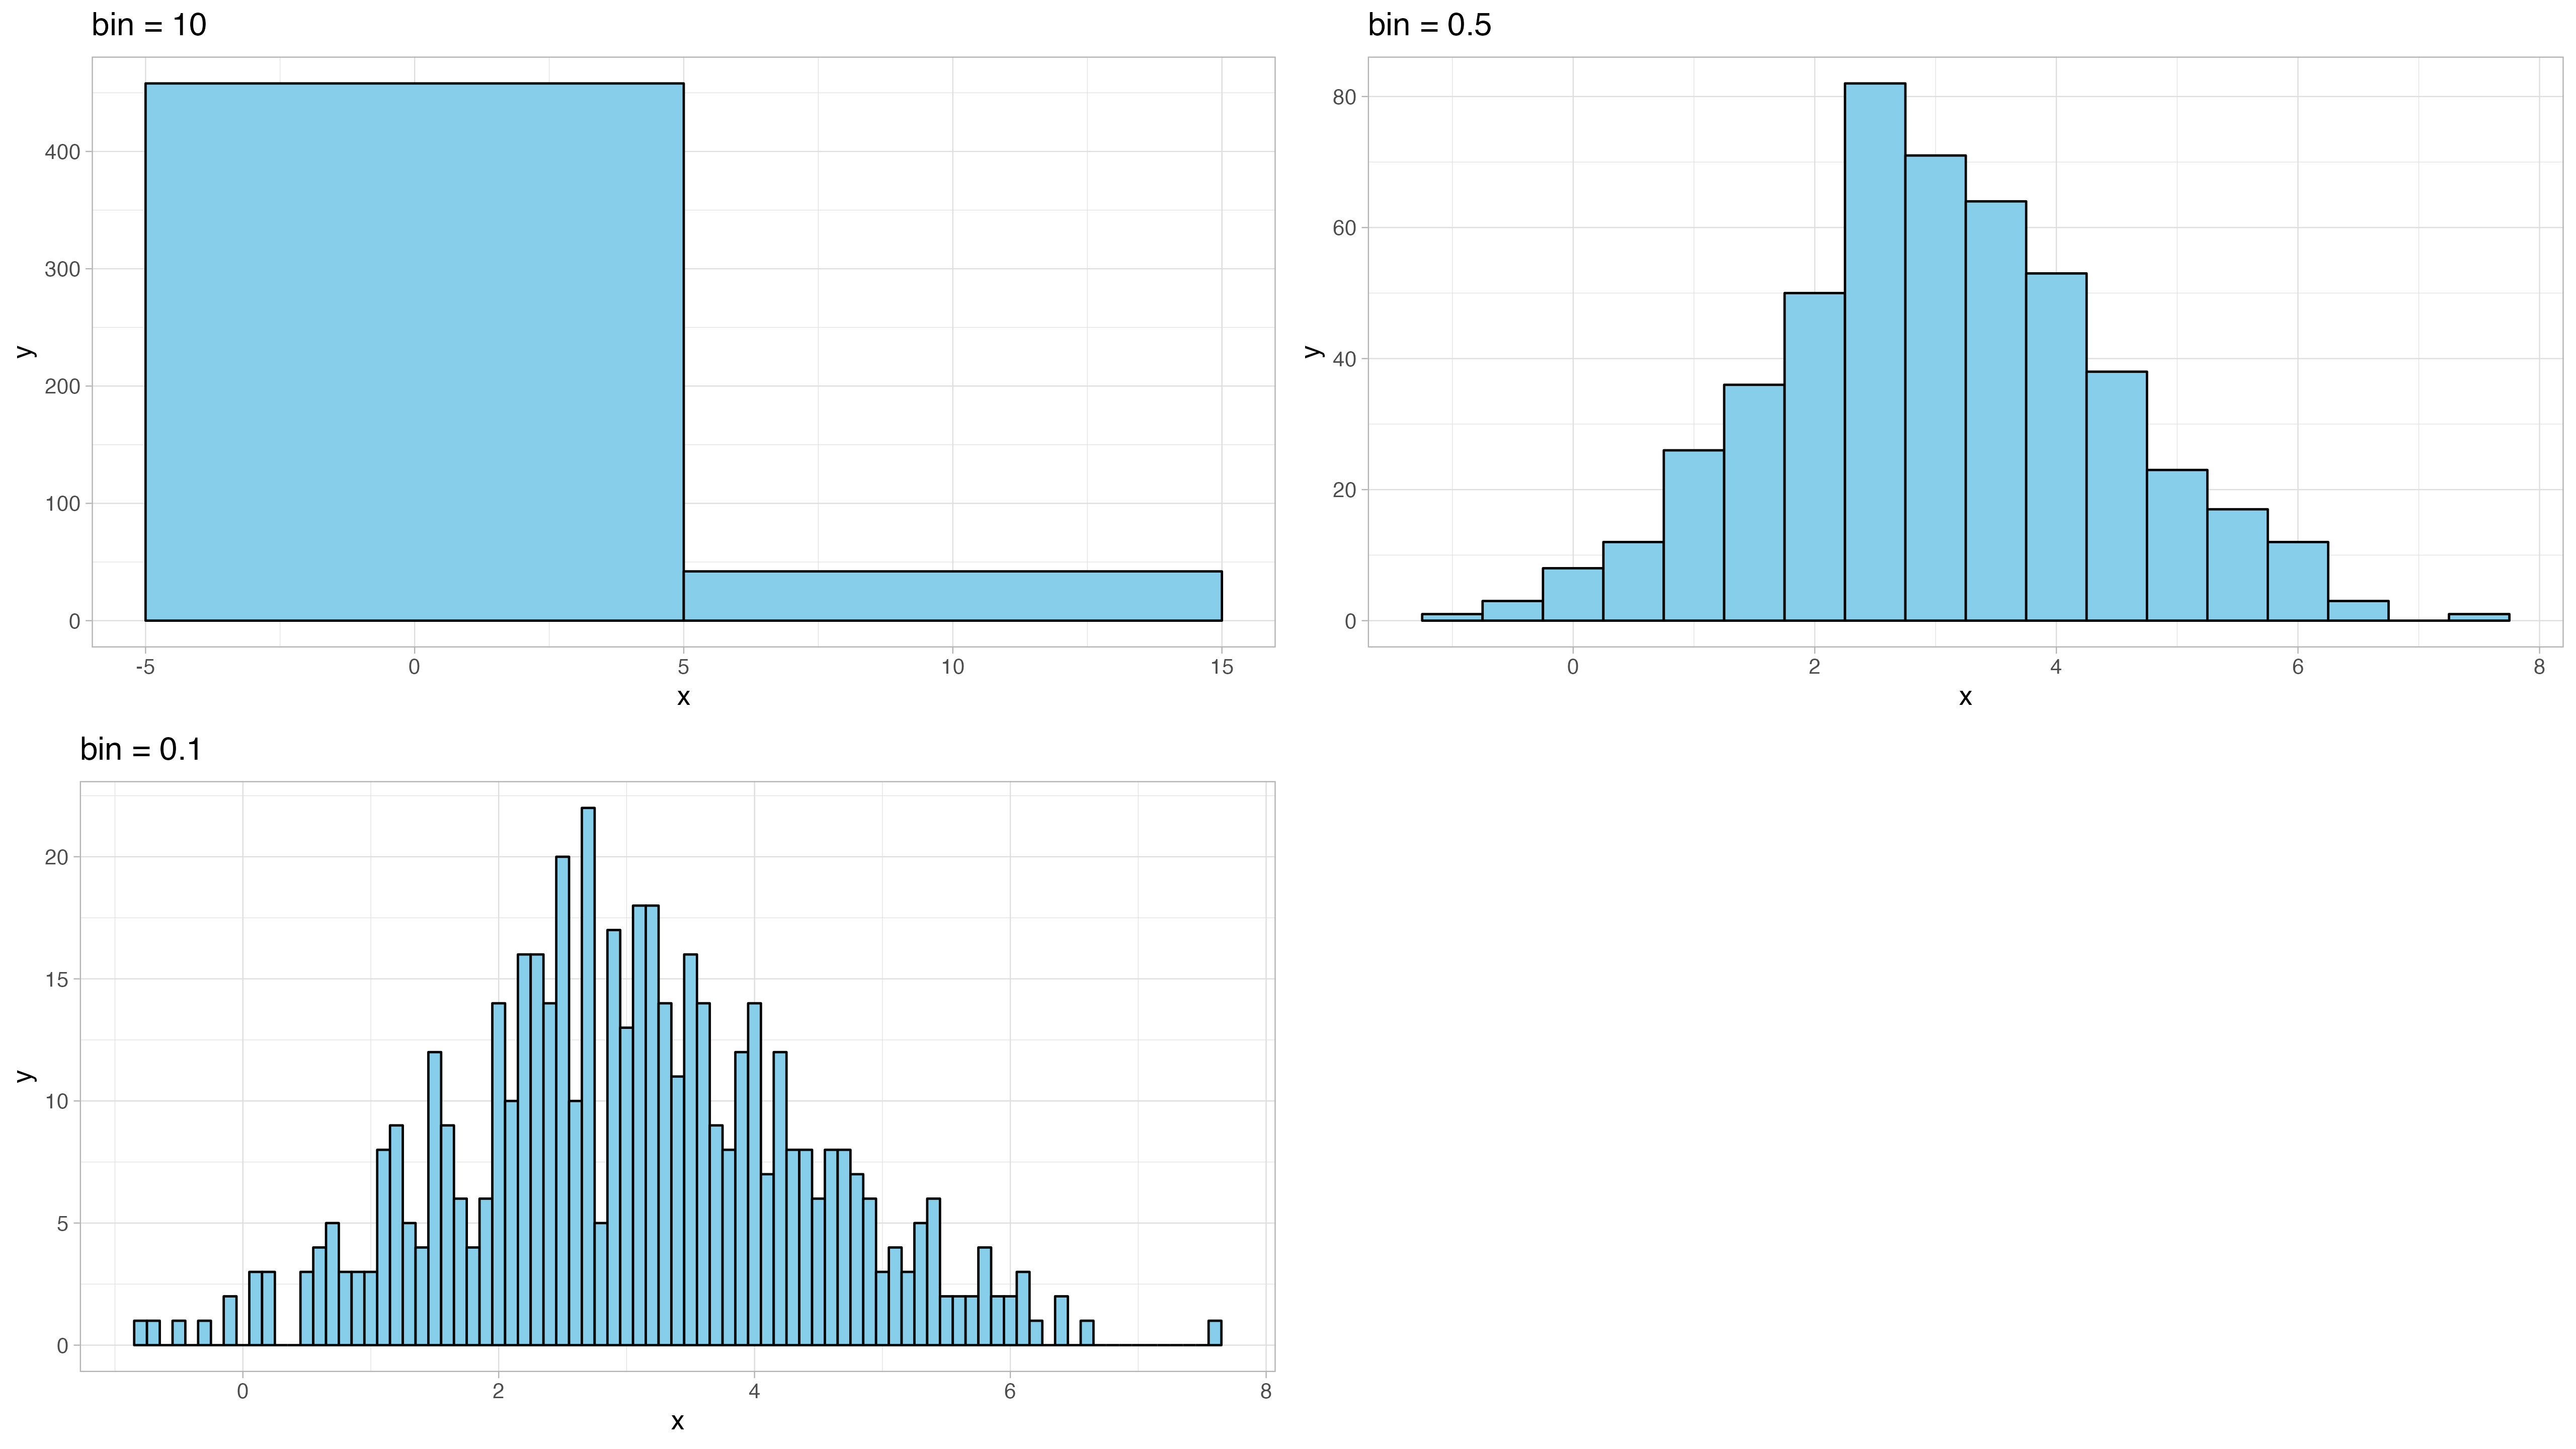
\includegraphics[width = \hsize]{\$HOME/code_box/learn/R/replication-project/src/analyze/output/figure/grid_hist.png}

\end{figure}

ヒストグラムはビンの幅によってデータの分布が著しく変わってしまう。運動神経 X のデータでヒストグラムを作成すると、bin = 10 のときは幅が大きすぎてデータの分布が見えにくく、bin = 0.1 のときは幅が小さすぎるためにヒストグラムが凸凹としていてデータの傾向がわかりにくい。このように、ヒストグラムで適切にデータの傾向を把握することは難しく、手動でビンの幅を何度も調整する必要がある。

\subsection {カーネル密度}
\begin{figure}[H]
  \centering
  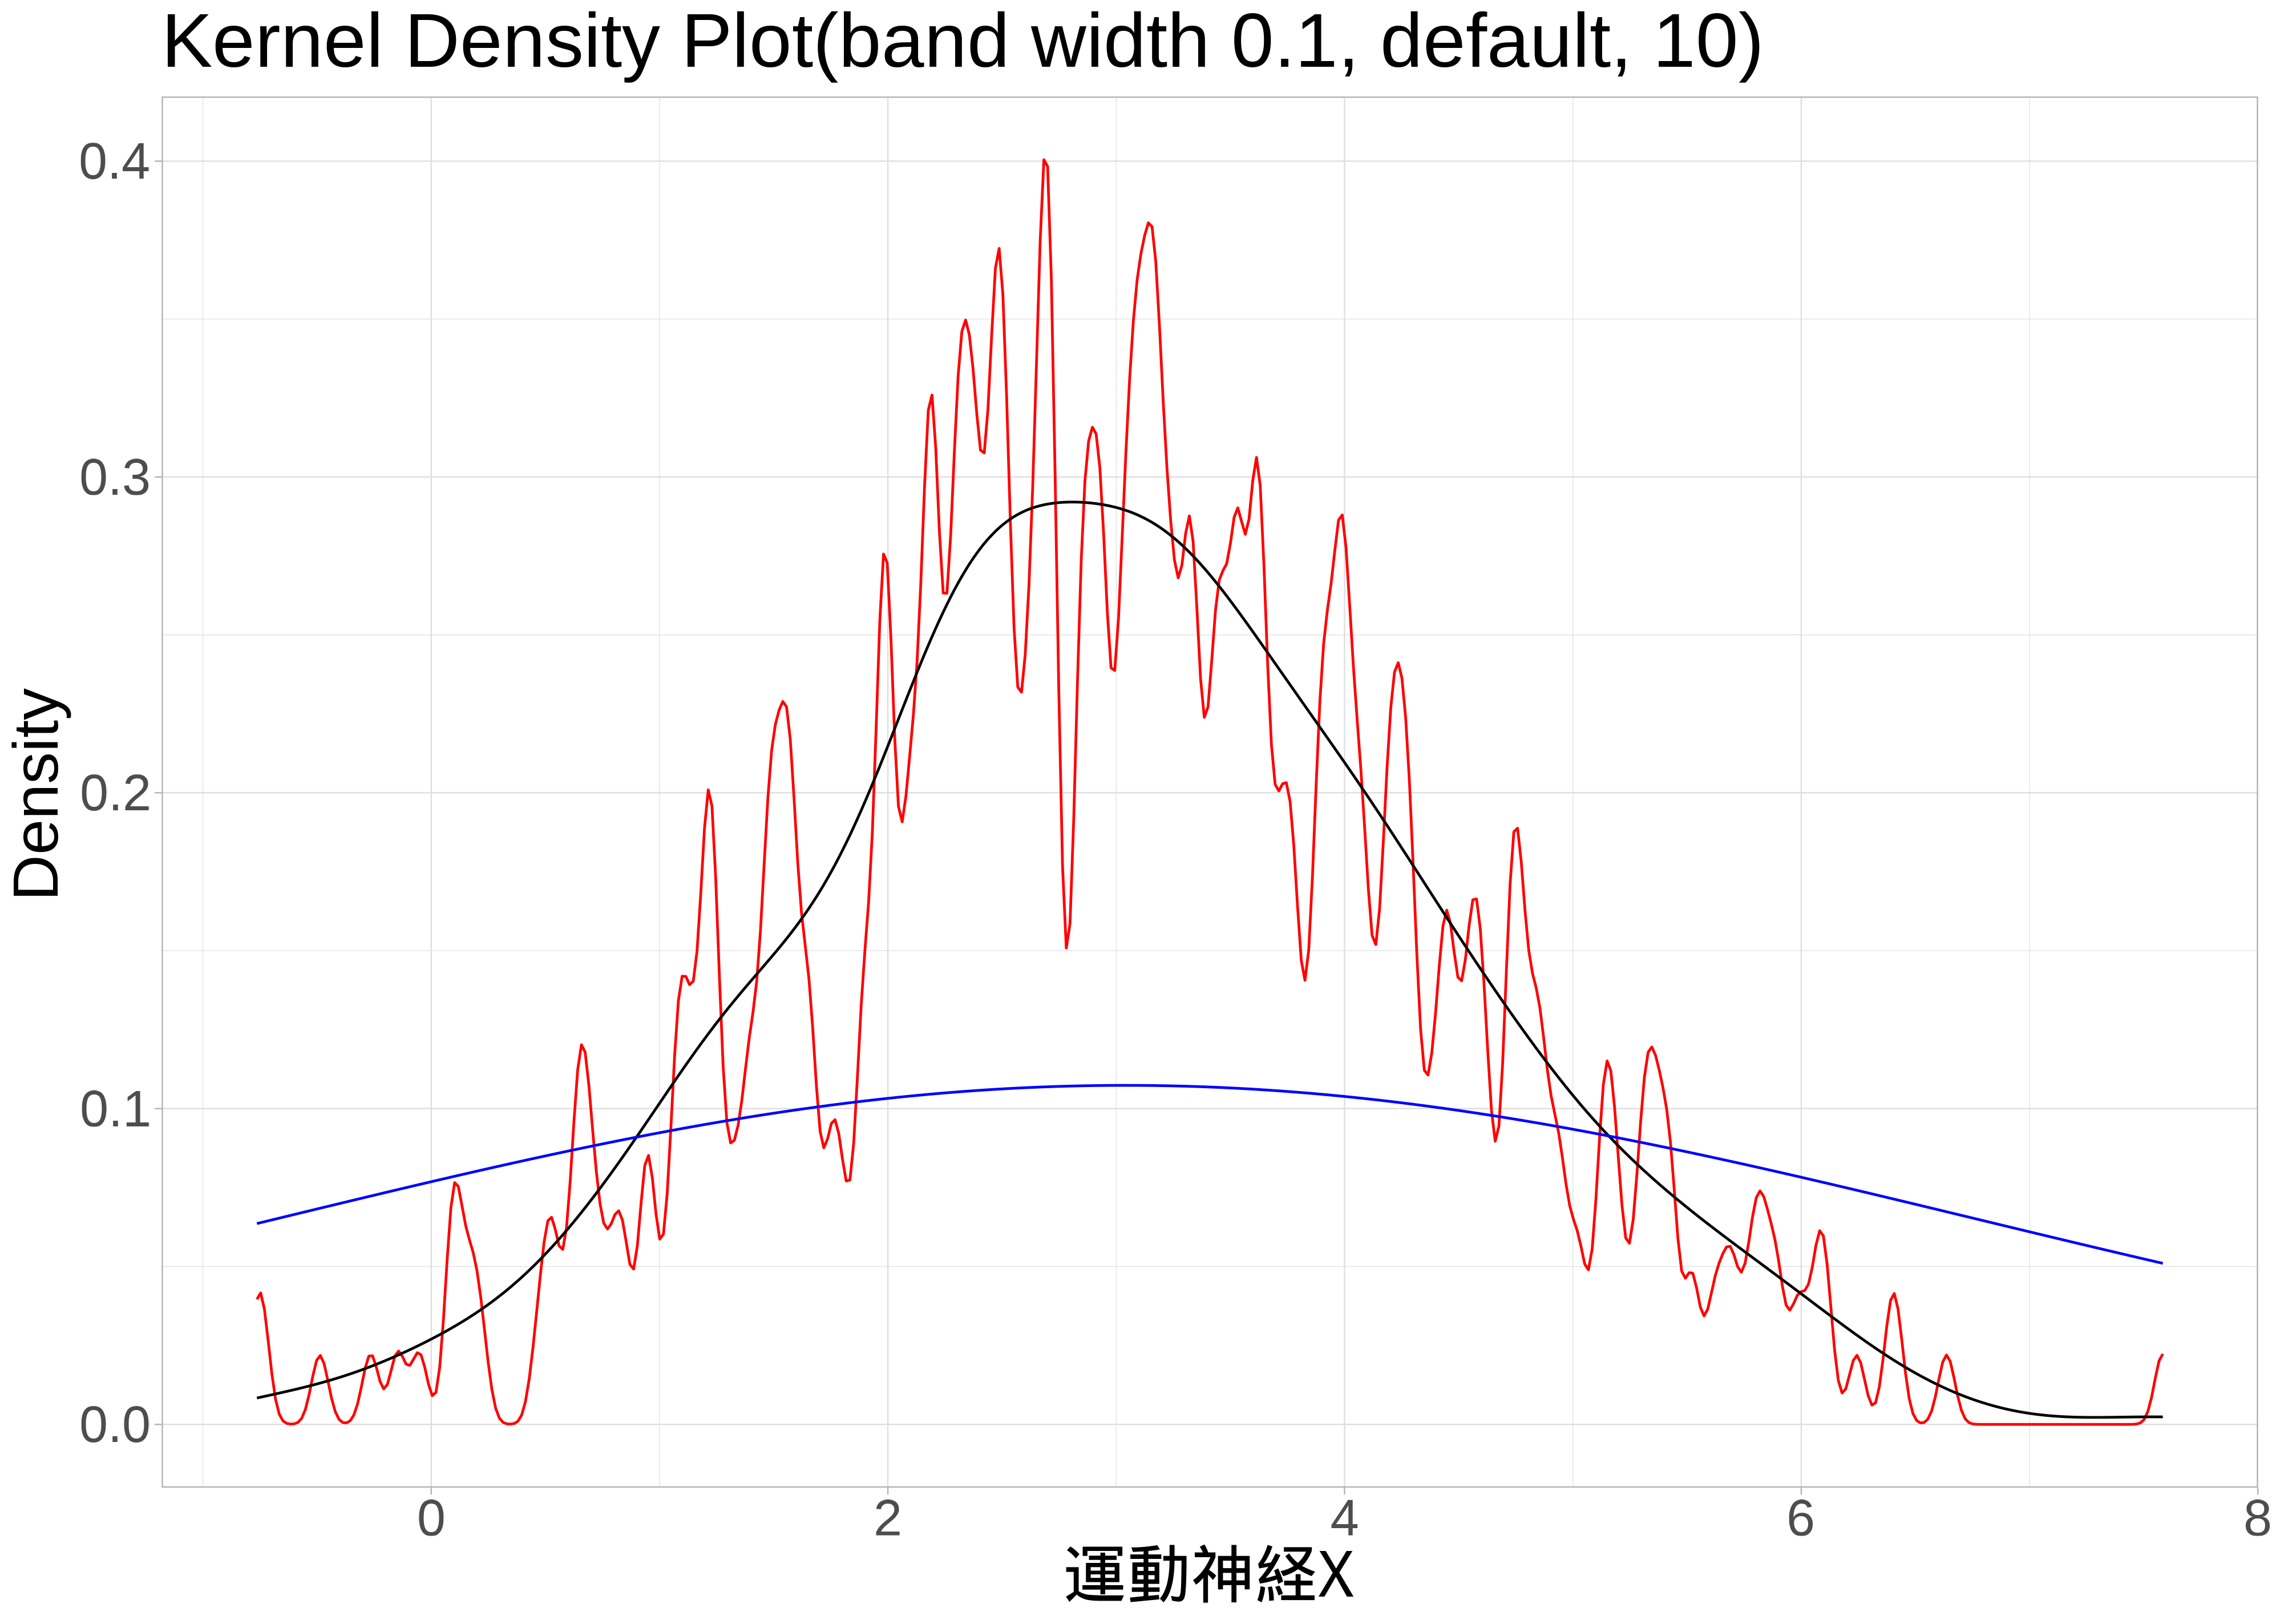
\includegraphics[width = \hsize]{\$HOME/code_box/learn/R/replication-project/src/analyze/output/figure/kernel_density.png}

\end{figure}

上図では、カーネルの幅を赤0.1, 黒デフォルト, 青10 として表時している。デフォルトが最も当てはまりが良いように見える。カーネル密度では、カーネルの幅が広がるほど曲線の滑らかさが増し広がりすぎるとデータの傾向が掴めなくなる。この傾向はヒストグラムがビンの幅を大きくするとデータの分布が見えにくくなることと似ている。

\subsection{分位回帰}

以下の回帰式を用いて、単回帰分析と分位回帰分析を行なった。

\begin{displaymath}
  \text{Z}_i = \beta_0 + \beta_1 \text{X}_i + \eta_i
\end{displaymath}

\begin{figure}[H]
  \centering
  
\begin{tabular}{l|r|r}
\hline
Model & Coefficient & Intercept\\
\hline
Simple Linear Regression & 1.896259 & 0.3226079\\
\hline
Quantile Regression (Median) & 1.899813 & 0.2702904\\
\hline
Quantile Regression (Q1) & 1.910714 & -0.7101449\\
\hline
Quantile Regression (Q3) & 1.859891 & 1.5548596\\
\hline
\end{tabular}

\end{figure}

単純な最小二乗法による回帰分析と、分位回帰の結果を表にまとめた。平均値と中央値を比較するとXの係数にさほどの違いはない。一方で、下位25\%のデータについては、Xの係数がおおきく、上位25\%のデータについては、Xの係数が小さい。

\end{document}
